\documentclass{ieeeaccess}
\usepackage{cite}
\usepackage{amsmath,amssymb,amsfonts}
\usepackage{graphicx}
\usepackage{textcomp}
\usepackage{bm}
\usepackage{booktabs}
\usepackage{multirow}
\usepackage{array}
\usepackage{url}
\def\UrlBreaks{\do\/\do-\do.\do_}

\makeatletter
\AtBeginDocument{\DeclareMathVersion{bold}
\SetSymbolFont{operators}{bold}{T1}{times}{b}{n}
\SetSymbolFont{NewLetters}{bold}{T1}{times}{b}{it}
\SetMathAlphabet{\mathrm}{bold}{T1}{times}{b}{n}
\SetMathAlphabet{\mathit}{bold}{T1}{times}{b}{it}
\SetMathAlphabet{\mathbf}{bold}{T1}{times}{b}{n}
\SetMathAlphabet{\mathtt}{bold}{OT1}{pcr}{b}{n}
\SetSymbolFont{symbols}{bold}{OMS}{cmsy}{b}{n}
\renewcommand\boldmath{\@nomath\boldmath\mathversion{bold}}}
\makeatother

\graphicspath{{figures/}}

\pdfinfo{
  /Title (An Empirical Evaluation of NVIDIA Kumo Tabular Against Traditional Machine Learning Models on Small Tabular Datasets)
  /Author (MD. Noyon Ahmed Joy, ORCID 0009-0004-9225-4610)
  /Subject (IEEE Access manuscript)
  /Keywords (Benchmarking, foundation models, gradient boosting, in-context learning, Kumo Tabular, small data, TabPFN, tabular data)
}

\begin{document}
\history{Date of publication xxxx 00, 0000, date of current version xxxx 00, 0000.}
\doi{10.1109/ACCESS.2024.0429000}

\title{An Empirical Evaluation of NVIDIA Kumo Tabular Against Traditional Machine Learning Models on Small Tabular Datasets}
\author{\uppercase{MD. Noyon Ahmed Joy}}
\address{Independent Researcher, Bangladesh (ORCID iD: 0009-0004-9225-4610, \url{https://orcid.org/0009-0004-9225-4610})}

\markboth
{Ahmed Joy: Empirical Evaluation of NVIDIA Kumo Tabular on Small Tabular Datasets}
{Ahmed Joy: Empirical Evaluation of NVIDIA Kumo Tabular on Small Tabular Datasets}

\corresp{Corresponding author: MD. Noyon Ahmed Joy (e-mail: noyonahmedjoyml@gmail.com).}

\tfootnote{This work did not receive any external funding.}

\begin{abstract}
Tabular foundation models predict the labels of new rows from labelled rows in a single forward pass, without training on the target dataset. This paper reports a controlled, reproducible comparison of NVIDIA Kumo Tabular, a recently released pretrained tabular transformer, with logistic or linear regression, random forests and histogram-based gradient boosting on two small public datasets: breast cancer diagnosis (569 rows, classification) and diabetes progression (442 rows, regression). All models share five random train/test splits and default settings, and are evaluated with standard metrics, runtime measurements, a paired statistical analysis that accounts for overlapping training sets, and a training-size study from 25 rows upwards. The smallest Kumo Tabular checkpoint obtained the best mean on every metric: accuracy 0.989 versus 0.977 for the strongest baseline, malignant-class recall 0.976 versus 0.948, and coefficient of determination 0.503 versus 0.496. In classification it matched or exceeded logistic regression on all five splits for every metric, but after correction for split overlap and multiple comparisons no difference is statistically significant at the 5\% level, and in regression the gap is within split-to-split variation. Kumo Tabular was markedly more robust than linear regression with 25 to 100 training rows, yet offered no advantage over logistic regression in classification at those sizes. Its prediction time per split was about 6 to 220 times that of the linear models across the hardware and runs measured. Kumo Tabular is a strong default for small tables, but on these benchmarks its advantage over well-chosen classical models is modest.
\end{abstract}

\begin{keywords}
Benchmarking, foundation models, gradient boosting, in-context learning, Kumo Tabular, small data, TabPFN, tabular data
\end{keywords}

\titlepgskip=-21pt

\maketitle

\section{Introduction}
\label{sec:introduction}
\PARstart{M}{ost} machine learning in industry and science is applied to tabular data, and for this setting tree ensembles and regularised linear models have remained the practical default for many years. Extensive comparisons found that gradient-boosted trees match or outperform deep neural networks on typical medium-sized tables \cite{shwartzziv2022tabular,grinsztajn2022tree,borisov2024survey}, although the gap depends strongly on the dataset \cite{mcelfresh2023neural} and on tuning \cite{kadra2021welltuned}.

Tabular foundation models change how a model is obtained. Instead of fitting parameters to the training split of each new dataset, a transformer is pretrained once on a large collection of tables and then conditions on the labelled rows of a new table at prediction time. TabPFN \cite{hollmann2023tabpfn,hollmann2025tabpfn} showed that a network pretrained on synthetic data can approximate Bayesian prediction for small tables, and later models extended the idea to larger inputs \cite{qu2025tabicl}. NVIDIA Kumo Tabular \cite{nvidia_kumo_card,nvidia_kumo_blog} is a recent, openly released model of this type. It is distributed through the \texttt{structured-data-models} library \cite{nvidia_sdm} in three sizes and, according to its developers, was pretrained only on synthetic tables.

Published claims about such models usually come from large benchmark suites evaluated by the model developers. Practitioners who consider adopting a pretrained tabular model for a small dataset face narrower questions: does it outperform the simple models they would otherwise use, is the difference larger than the noise of a small test set, and what does it cost? This paper addresses these questions for Kumo Tabular on two well-known datasets. It makes the following contributions:
\begin{itemize}
\item A reproducible comparison of Kumo Tabular with three classical baselines on identical splits, including classification, regression, a training-size study and runtime measurements. Code, results and notebooks are public \cite{project_repo,project_kaggle}.
\item A paired statistical analysis that accounts for the dependence between resampled splits \cite{nadeau2003inference} and for multiple comparisons \cite{holm1979}, together with an explicit statement of what five splits can and cannot establish.
\item An analysis of where the pretrained model helps (classification recall, very small regression training sets, built-in predictive intervals) and where it does not (small classification training sets, the full regression task, prediction cost).
\end{itemize}

The study is deliberately small in scope. It does not attempt a general ranking of tabular methods, and the medical datasets are used as standard benchmarks only; nothing in this paper should be read as evidence of clinical reliability.

\section{Related Work}

\subsection{Classical models for tabular data}
Logistic regression \cite{cox1958logistic} and ordinary least squares remain strong baselines for small, low-dimensional problems. Random forests \cite{breiman2001rf} average decorrelated decision trees, and gradient boosting \cite{friedman2001gbm} fits trees sequentially to the residuals of the current ensemble; efficient implementations such as XGBoost \cite{chen2016xgboost}, LightGBM \cite{ke2017lightgbm} and CatBoost \cite{prokhorenkova2018catboost} made boosting the default for many tabular tasks. Scikit-learn \cite{pedregosa2011sklearn} provides the implementations used in this study, including a histogram-based boosting estimator in the style of LightGBM.

\subsection{Deep learning on tables}
Neural architectures designed for tables, such as TabNet \cite{arik2021tabnet} and transformer variants \cite{gorishniy2021revisiting}, have been compared extensively with tree ensembles. Surveys and benchmarks report that trees remain competitive or superior on many medium-sized datasets \cite{shwartzziv2022tabular,borisov2024survey,grinsztajn2022tree}, that well-regularised multilayer perceptrons can close the gap \cite{kadra2021welltuned}, and that the best family varies across datasets, with dataset properties mattering more than the choice between neural networks and boosted trees \cite{mcelfresh2023neural}.

\subsection{In-context learning}
In-context learning describes a pretrained model solving a new task from examples supplied in its input, without updating its weights. It was popularised by large language models \cite{brown2020gpt3}, which build on the transformer architecture \cite{vaswani2017attention}, and has been shown to emerge for simple function classes when transformers are trained on suitable task distributions \cite{garg2022icl}. Large language models have also been applied directly to serialised tables \cite{hegselmann2023tabllm}.

\subsection{Tabular foundation models}
Prior-data fitted networks (PFNs) \cite{muller2022pfn} are transformers trained on datasets sampled from a prior so that a single forward pass approximates the posterior predictive distribution. TabPFN \cite{hollmann2023tabpfn} applied this to small classification tables using priors based on structural causal models, and its successor \cite{hollmann2025tabpfn} added regression, larger inputs and a two-way attention over rows and columns. TabICL \cite{qu2025tabicl} compresses each row into a fixed-size embedding with column- and row-wise attention before in-context learning, which allows much larger tables. Set-based attention with inducing points \cite{lee2019set} is a common building block for processing columns efficiently.

\subsection{NVIDIA Kumo Tabular}
Kumo Tabular \cite{nvidia_kumo_card,nvidia_kumo_blog} follows this line of work. Its developers describe it as a transformer with column, row and in-context attention ``as introduced in TabICL and TabPFN'', pretrained entirely on synthetic tables sampled from structural causal models, released in three sizes with 28M to 215M parameters under the OpenMDW 1.1 licence. They report first places on several public benchmark suites \cite{nvidia_kumo_blog}; those claims are the developers' own and are not evaluated here. To the best of the author's knowledge, no independent evaluation of Kumo Tabular on these two datasets had been published at the time of writing.

\section{Background: Training Versus In-Context Learning}
\label{sec:background}

Let $\mathcal{D}_{\mathrm{tr}}=\{(\mathbf{x}_i,y_i)\}_{i=1}^{n}$ be a labelled training set and $\mathbf{x}_q$ a query row.

\subsection{Conventional supervised learning}
A classical model chooses parameters by (regularised) empirical risk minimisation on the dataset at hand,
\begin{equation}
\hat{\boldsymbol\theta}=\arg\min_{\boldsymbol\theta}\;\frac{1}{n}\sum_{i=1}^{n}\ell\big(f_{\boldsymbol\theta}(\mathbf{x}_i),y_i\big)+\lambda\,\Omega(\boldsymbol\theta),
\label{eq:erm}
\end{equation}
and predicts $\hat{y}_q=f_{\hat{\boldsymbol\theta}}(\mathbf{x}_q)$. The cost of~\eqref{eq:erm} is paid once per dataset; afterwards predictions are cheap and independent of $n$.

\subsection{Pretrained in-context learning}
A tabular foundation model has parameters $\boldsymbol\phi$ that were fitted once, before the target dataset was seen, by minimising the expected predictive loss over many datasets $\mathcal{D}$ drawn from a generator $p(\mathcal{D})$:
\begin{equation}
\boldsymbol\phi^{\star}=\arg\min_{\boldsymbol\phi}\;\mathbb{E}_{\mathcal{D}\sim p(\mathcal{D})}\Big[-\log q_{\boldsymbol\phi}\big(y_q\mid\mathbf{x}_q,\mathcal{D}_{\mathrm{ctx}}\big)\Big],
\label{eq:pfn}
\end{equation}
where each sampled dataset is split into context rows $\mathcal{D}_{\mathrm{ctx}}$ and held-out query rows. For a sufficiently expressive model, $q_{\boldsymbol\phi}$ approximates the posterior predictive distribution $p(y_q\mid\mathbf{x}_q,\mathcal{D}_{\mathrm{ctx}})=\int p(y_q\mid\mathbf{x}_q,\psi)\,p(\psi\mid\mathcal{D}_{\mathrm{ctx}})\,d\psi$ implied by the generator \cite{muller2022pfn}. On a new dataset, $\boldsymbol\phi^{\star}$ stays fixed and the training split is supplied as context:
\begin{equation}
\hat{p}(y_q\mid\mathbf{x}_q)=q_{\boldsymbol\phi^{\star}}\big(y_q\mid\mathbf{x}_q,\mathcal{D}_{\mathrm{tr}}\big).
\label{eq:icl}
\end{equation}
No gradient step is taken on $\mathcal{D}_{\mathrm{tr}}$. Everything the model ``learns'' about the dataset happens inside the forward pass, through attention from query rows to context rows. Fig.~\ref{fig:paradigms} contrasts the two procedures. Two practical consequences follow. First, there is no separate training stage to tune or validate. Second, every prediction call must process the context again; there is no compact fitted model that can be applied later at negligible cost, unless context representations are cached.

\begin{figure}[t]
\centering
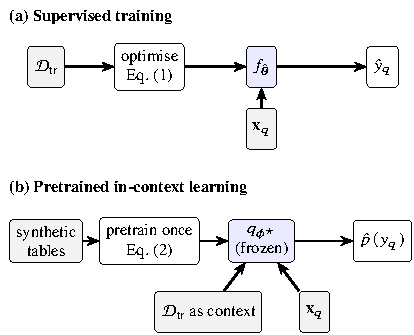
\includegraphics[width=\columnwidth]{paradigms_diagram.pdf}
\caption{Conventional supervised learning fits parameters to each dataset (a). A tabular foundation model is pretrained once on synthetic datasets and conditions on the labelled rows of a new dataset at prediction time, without updating its weights (b).}
\label{fig:paradigms}
\end{figure}

\subsection{Kumo Tabular as used in this study}
The following description is taken from the developers' documentation \cite{nvidia_kumo_blog} and the source code of \texttt{structured-data-models} 0.2.1 \cite{nvidia_sdm}. Cell values are embedded with learned Fourier features and grouped into tokens. A row encoder alternates column-wise induced self-attention, in which every row attends only to context rows, with row-wise attention across the tokens of one row; four readout tokens summarise each row into a fixed-size embedding. A final transformer performs in-context learning over row embeddings, with context rows attending to each other and query rows attending to context rows only. The classification head outputs class scores for up to ten classes; the library wraps it in an error-correcting output code scheme \cite{dietterich1995ecoc}. The regression head outputs 999 quantiles $q_{\tau}$, $\tau\in\{0.001,\dots,0.999\}$ \cite{koenker1978quantiles}.

A built-in preprocessing recipe creates an ensemble of $E$ views of the table. Each view standardises the features and applies one of four transformations (identity, power transform, robust scaling with soft clipping, or rank-Gaussian), shuffles the column order, and, for classification, cyclically shifts the class labels. For classification, the estimator outputs $\mathbf{z}_e$ are averaged and normalised,
\begin{equation}
\hat{\mathbf{p}}=\operatorname{softmax}\Big(\frac{1}{E}\sum_{e=1}^{E}\mathbf{z}_e\Big),\qquad \hat{y}=\arg\max_{k}\hat{p}_k ;
\label{eq:ensemble}
\end{equation}
for regression, each estimator's quantiles are sorted and combined with a 20\% trimmed mean. This study uses the \texttt{small} checkpoints (27.5M parameters for classification and 28.5M for regression, counted from the loaded models) with $E=8$.

\section{Methodology}

\subsection{Datasets}
Both datasets ship with scikit-learn and are summarised in Table~\ref{tab:datasets}. The Breast Cancer Wisconsin (Diagnostic) dataset \cite{street1993nuclear} contains 30 numerical features computed from digitised images of fine-needle aspirates. The label was recoded so that malignant tumours form the positive class, because missed malignant cases are the costly error. The diabetes dataset \cite{efron2004lars} contains ten baseline variables and a quantitative measure of disease progression one year later; features were used in their original units rather than the default standardised version.

\begin{table}[t]
\centering
\caption{Datasets used in the study.}
\label{tab:datasets}
\setlength{\tabcolsep}{4pt}
\begin{tabular}{lcc}
\toprule
& Breast cancer \cite{street1993nuclear} & Diabetes \cite{efron2004lars} \\
\midrule
Task & binary classification & regression \\
Rows & 569 & 442 \\
Features & 30 numerical & 10 numerical \\
Target & 212 malignant, 357 benign & progression, 25 to 346 \\
Train / test rows & 455 / 114 & 353 / 89 \\
Split & stratified 80/20 & random 80/20 \\
\bottomrule
\end{tabular}
\end{table}

\subsection{Experimental protocol}
Each experiment is repeated over five train/test partitions generated with seeds 42 to 46 (stratified for classification). Within a seed, every model receives the identical partition. For Kumo Tabular, the training rows with their targets form the context, and the test rows without the target column form the query. The implementation rejects query tables that contain the target, checks that training and test rows are disjoint, and validates the length and finiteness of all predictions before metrics are computed. If Kumo Tabular fails to load or run, its results are recorded as incomplete rather than replaced; this did not occur in the reported runs.

\subsection{Models and configuration}
Table~\ref{tab:models} lists the models. All baselines use scikit-learn defaults with a fixed random state; logistic regression receives standardised inputs, and random forests use 500 trees. No model is tuned, so the comparison is between out-of-the-box methods. Kumo Tabular uses the \texttt{small} checkpoint, eight ensemble members, an estimator batch size of one and a seeded random number generator, which makes its predictions deterministic for a given split. For regression, the median $q_{0.5}$ is the point prediction and $[q_{0.05},q_{0.95}]$ a nominal 90\% predictive interval.

\begin{table}[t]
\centering
\caption{Models and settings. All models use the same splits; none is tuned.}
\label{tab:models}
\setlength{\tabcolsep}{3pt}
\begin{tabular}{>{\raggedright\arraybackslash}p{0.24\columnwidth}>{\raggedright\arraybackslash}p{0.68\columnwidth}}
\toprule
Model & Configuration \\
\midrule
Kumo Tabular & \texttt{small} checkpoint, $E=8$ estimators, seeded; median quantile for regression \\
Logistic Reg. & standardisation, L2 penalty $C=1$, \texttt{max\_iter}=5000 \\
Linear Reg. & ordinary least squares \\
Random Forest & 500 trees, default depth and features \\
HistGB & histogram gradient boosting, defaults (100 iterations, min.\ 20 samples per leaf) \\
\bottomrule
\end{tabular}
\end{table}

\subsection{Evaluation metrics}
For classification with true positives $TP$, false positives $FP$, true negatives $TN$ and false negatives $FN$, the study reports
\begin{gather}
\mathrm{Precision}=\tfrac{TP}{TP+FP},\qquad \mathrm{Recall}=\tfrac{TP}{TP+FN},\\
F_1=\tfrac{2\,\mathrm{Precision}\cdot\mathrm{Recall}}{\mathrm{Precision}+\mathrm{Recall}},
\end{gather}
accuracy $(TP+TN)/m$ on $m$ test rows, the area under the ROC curve \cite{fawcett2006roc} and the confusion matrix. Class predictions use the arg-max rule~\eqref{eq:ensemble}, equivalent to a 0.5 threshold. For regression with predictions $\hat{y}_j$,
\begin{gather}
\mathrm{MAE}=\tfrac{1}{m}\textstyle\sum_j|y_j-\hat{y}_j|,\quad
\mathrm{RMSE}=\sqrt{\tfrac{1}{m}\textstyle\sum_j(y_j-\hat{y}_j)^2},\\
R^2=1-\frac{\sum_j(y_j-\hat{y}_j)^2}{\sum_j(y_j-\bar{y})^2}.
\end{gather}
Interval quality is measured by the mean interval width and the empirical coverage
\begin{equation}
\mathrm{Coverage}=\frac{1}{m}\sum_{j=1}^{m}\mathbf{1}\big[q_{0.05,j}\le y_j\le q_{0.95,j}\big],
\end{equation}
where $\mathbf{1}[\cdot]$ is the indicator function.

\subsection{Runtime measurement}
Runtime is the wall-clock fit time plus prediction time per split. Kumo Tabular has no fitting stage, so its full cost is counted as prediction time. One warm-up call on training rows precedes timing to exclude one-off CUDA initialisation. Kumo Tabular ran on the GPU and the baselines on the CPU (Table~\ref{tab:environment}); runtimes therefore compare complete pipelines on the available hardware, not algorithms on equal hardware.

\begin{table}[t]
\centering
\caption{Computational environment.}
\label{tab:environment}
\setlength{\tabcolsep}{3pt}
\begin{tabular}{ll}
\toprule
GPU & NVIDIA GeForce GTX 980M, 8\,GB (compute capability 5.2) \\
CPU & Intel Core i7-6700HQ, 4 cores, 8 threads \\
OS & Windows 10 \\
Software & Python 3.12.16, PyTorch 2.14.1 (CUDA 12.6) \cite{paszke2019pytorch}, \\
& structured-data-models 0.2.1, scikit-learn 1.9.1 \\
Precision & float32; float16 autocast disabled (GPU older than 7.0) \\
\bottomrule
\end{tabular}
\end{table}

\subsection{Statistical analysis}
\label{sec:stats}
For each metric, the paired advantage of Kumo Tabular over the strongest baseline on split $s$ is $d_s$, signed so that $d_s>0$ favours Kumo for every metric. With $k=5$ splits, mean $\overline{d}$ and standard deviation $s_d$, the usual paired $t$-test treats the $d_s$ as independent. They are not: the training sets of different splits overlap heavily, which makes the naive test anti-conservative \cite{dietterich1998tests}. The study therefore also reports the corrected resampled $t$-statistic of Nadeau and Bengio \cite{nadeau2003inference},
\begin{equation}
t_{\mathrm{corr}}=\frac{\overline{d}}{\sqrt{\left(\frac{1}{k}+\frac{n_{\mathrm{te}}}{n_{\mathrm{tr}}}\right)s_d^{2}}},
\label{eq:corrected}
\end{equation}
with $k-1$ degrees of freedom and $n_{\mathrm{te}}/n_{\mathrm{tr}}\approx0.25$, the corresponding 95\% confidence interval, and Holm's step-down adjustment \cite{holm1979} across the metrics of each task. As a distribution-free check, the exact Wilcoxon signed-rank test \cite{wilcoxon1945} is given; with five non-zero differences its smallest attainable two-sided $p$-value is $2/2^5=0.0625$, so it cannot reach the 5\% level in this design. Counts of wins, ties and losses are reported descriptively \cite{demsar2006comparisons}.

\subsection{Training-size study}
To examine the small-data regime, the training split of seeds 42 to 44 is subsampled (stratified for classification) to 25, 50, 100 and 200 rows, plus 400 rows for classification and the full training set. All models receive the same subsample, and evaluation always uses the complete test split of the seed.

\section{Results}

\subsection{Classification}
Table~\ref{tab:classification} summarises the breast cancer results. Kumo Tabular obtained the highest mean on all five metrics, followed by logistic regression; the tree ensembles were clearly behind. The largest difference is in recall: pooled over the five test sets, which contain 210 malignant and 360 benign cases in total, Kumo Tabular missed 5 malignant tumours and produced 1 false alarm, compared with 11 and 2 for logistic regression, 14 and 5 for histogram gradient boosting, and 15 and 11 for random forests. Fig.~\ref{fig:confusion} shows the confusion matrices for the first split. ROC-AUC is close to saturation for all models (0.988 to 0.998), so the ROC and precision-recall curves in Fig.~\ref{fig:roc} separate the models less than recall does.

\begin{table*}[t]
\centering
\caption{Breast cancer classification results (mean $\pm$ standard deviation over five stratified splits, 114 test rows each). Malignant is the positive class. Time is fit plus prediction time per split. Best mean per metric in bold.}
\label{tab:classification}
\setlength{\tabcolsep}{5pt}
\begin{tabular}{lcccccc}
\toprule
Model & Accuracy & Precision & Recall & F1 & ROC-AUC & Time (s) \\
\midrule
Kumo Tabular & \textbf{0.989 $\pm$ 0.010} & \textbf{0.995 $\pm$ 0.010} & \textbf{0.976 $\pm$ 0.029} & \textbf{0.985 $\pm$ 0.014} & \textbf{0.998 $\pm$ 0.003} & 1.099 $\pm$ 0.012 \\
Logistic Reg. & 0.977 $\pm$ 0.012 & 0.990 $\pm$ 0.013 & 0.948 $\pm$ 0.031 & 0.968 $\pm$ 0.017 & 0.995 $\pm$ 0.004 & 0.019 $\pm$ 0.001 \\
Random Forest & 0.954 $\pm$ 0.013 & 0.947 $\pm$ 0.031 & 0.929 $\pm$ 0.024 & 0.938 $\pm$ 0.018 & 0.988 $\pm$ 0.011 & 1.204 $\pm$ 0.063 \\
HistGB & 0.967 $\pm$ 0.016 & 0.976 $\pm$ 0.024 & 0.933 $\pm$ 0.043 & 0.953 $\pm$ 0.022 & 0.994 $\pm$ 0.007 & 0.274 $\pm$ 0.020 \\
\bottomrule
\end{tabular}
\end{table*}


\begin{figure*}[t]
\centering
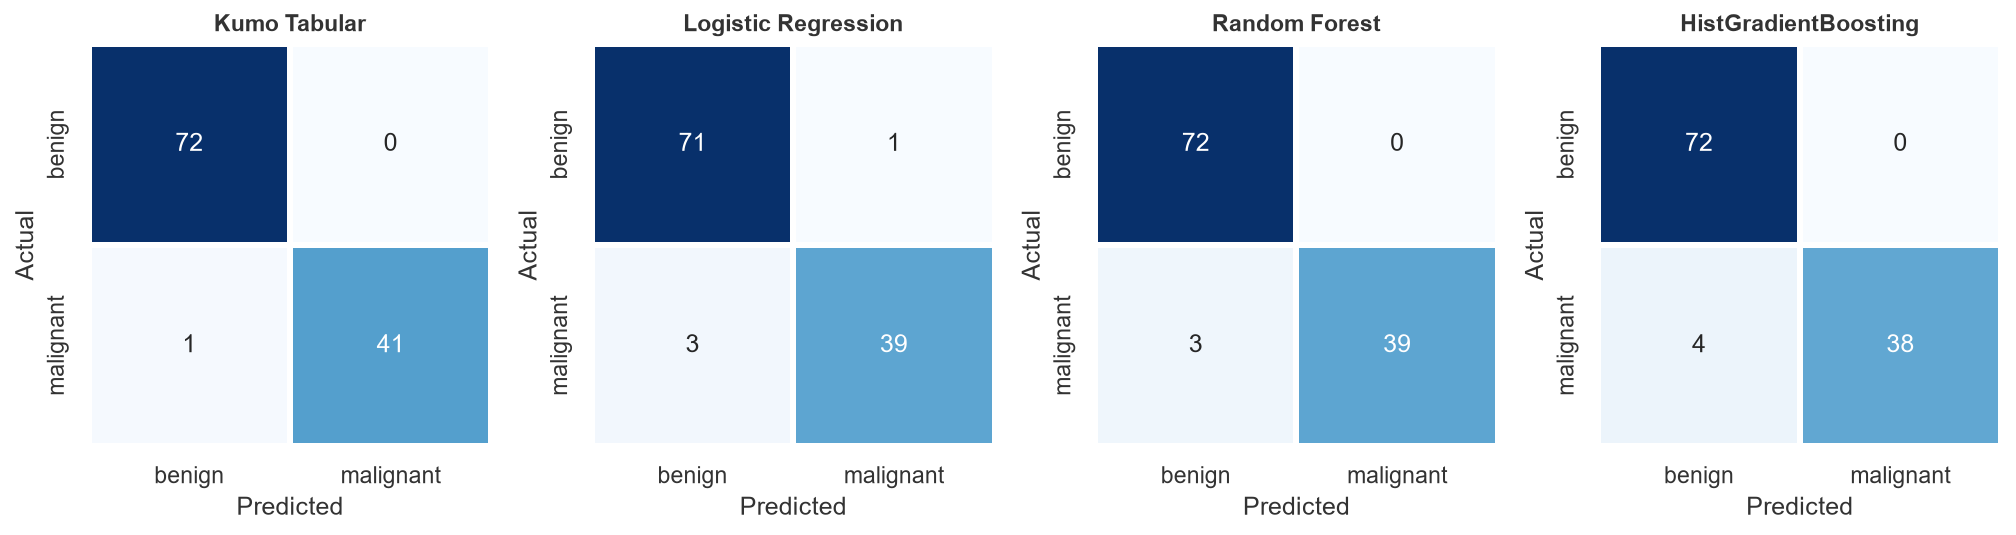
\includegraphics[width=0.86\textwidth]{classification_confusion_matrices.png}
\caption{Confusion matrices on the first classification split (seed 42, 72 benign and 42 malignant test cases).}
\label{fig:confusion}
\end{figure*}

\begin{figure*}[t]
\centering
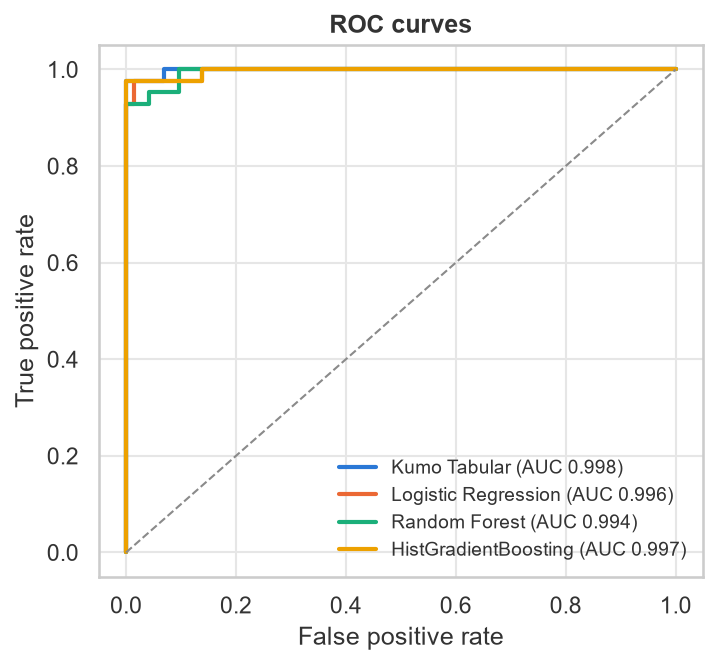
\includegraphics[width=0.40\textwidth]{classification_roc_curves.png}\hspace{0.04\textwidth}
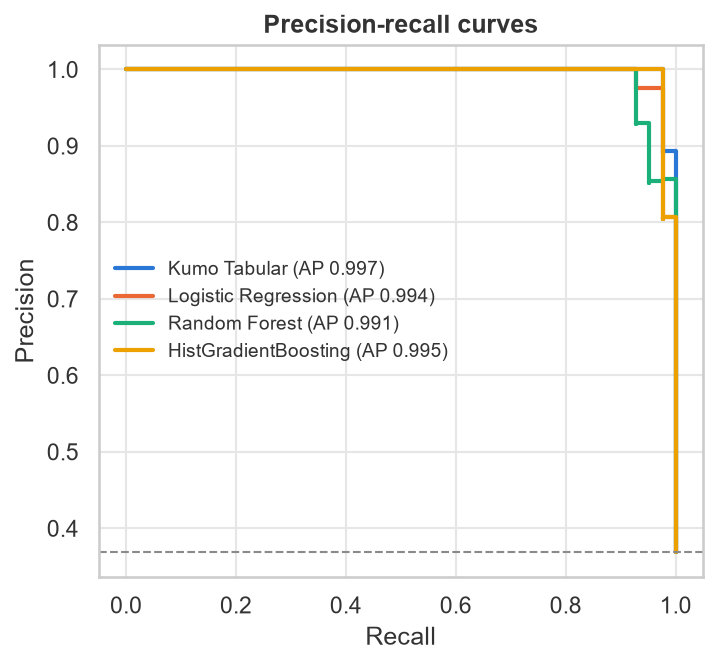
\includegraphics[width=0.40\textwidth]{classification_precision_recall.png}
\caption{ROC curves (left) and precision-recall curves (right) on the first classification split. AP denotes average precision; the dashed lines mark a random classifier.}
\label{fig:roc}
\end{figure*}

\subsection{Regression}
Table~\ref{tab:regression} reports the diabetes results. Kumo Tabular again had the best means, but linear regression was close behind on every metric, and both were clearly better than the tree ensembles. Fig.~\ref{fig:actual} plots predictions against targets for the first split and Fig.~\ref{fig:residuals} the residual distributions. The patterns of Kumo Tabular and linear regression are similar; on that split, their absolute errors had a Pearson correlation of 0.93, compared with 0.76 and 0.72 between Kumo Tabular and the random forest and boosting models. The largest errors are shared across models, which points to noise in the target rather than a weakness of one method.

\begin{table*}[t]
\centering
\caption{Diabetes regression results (mean $\pm$ standard deviation over five random splits, 89 test rows each). Kumo Tabular uses the median quantile $q_{0.5}$ as point prediction. Best mean per metric in bold.}
\label{tab:regression}
\setlength{\tabcolsep}{5pt}
\begin{tabular}{lcccc}
\toprule
Model & MAE & RMSE & $R^2$ & Time (s) \\
\midrule
Kumo Tabular & \textbf{42.48 $\pm$ 3.10} & \textbf{52.88 $\pm$ 3.47} & \textbf{0.503 $\pm$ 0.039} & 0.627 $\pm$ 0.053 \\
Linear Reg. & 43.75 $\pm$ 3.59 & 53.27 $\pm$ 4.03 & 0.496 $\pm$ 0.046 & 0.003 $\pm$ 0.000 \\
Random Forest & 45.23 $\pm$ 2.63 & 56.16 $\pm$ 3.31 & 0.440 $\pm$ 0.022 & 0.833 $\pm$ 0.024 \\
HistGB & 45.85 $\pm$ 0.72 & 58.52 $\pm$ 1.67 & 0.390 $\pm$ 0.042 & 0.190 $\pm$ 0.031 \\
\bottomrule
\end{tabular}
\end{table*}


\begin{figure*}[t]
\centering
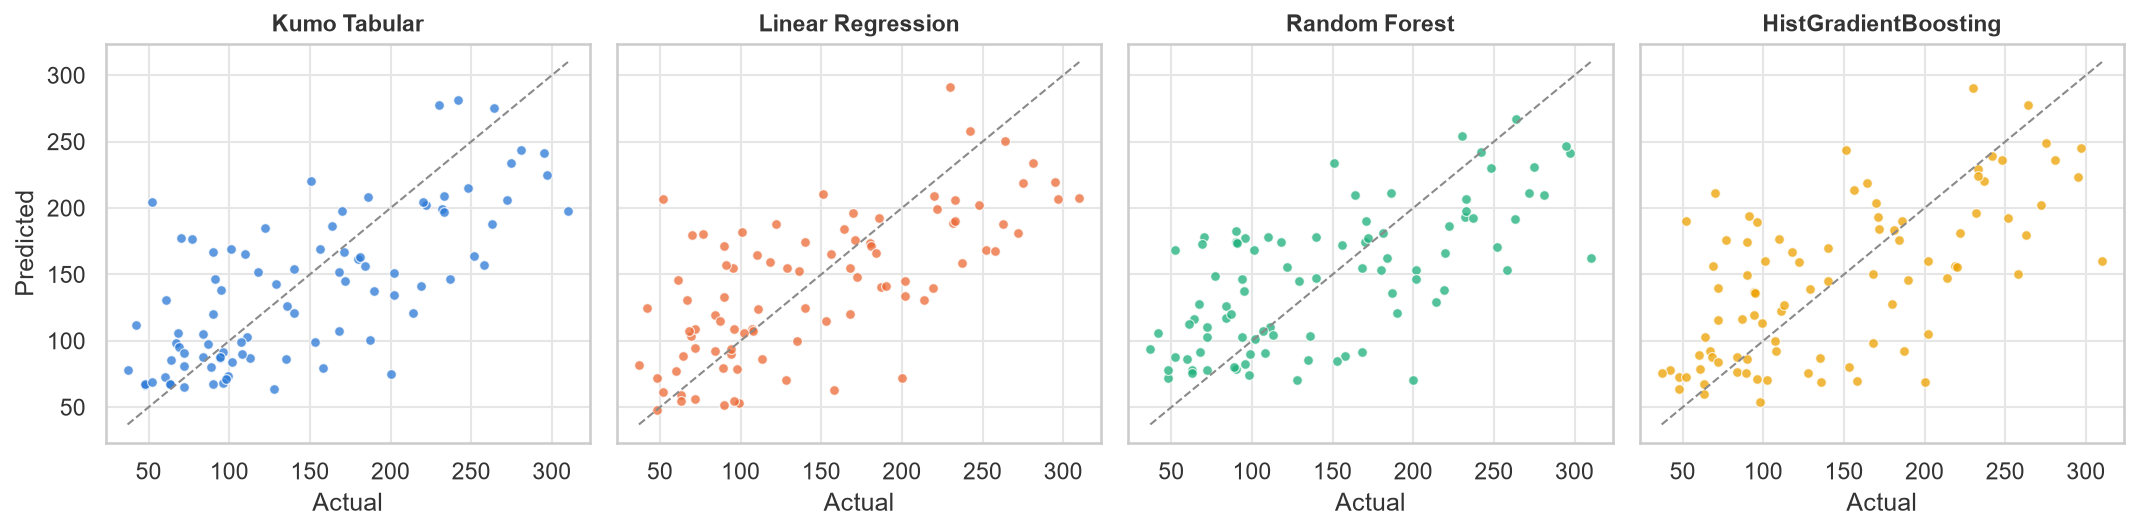
\includegraphics[width=0.92\textwidth]{regression_actual_vs_predicted.png}
\caption{Predicted versus actual disease progression on the first regression split (seed 42). The dashed line marks perfect prediction.}
\label{fig:actual}
\end{figure*}

\begin{figure*}[t]
\centering
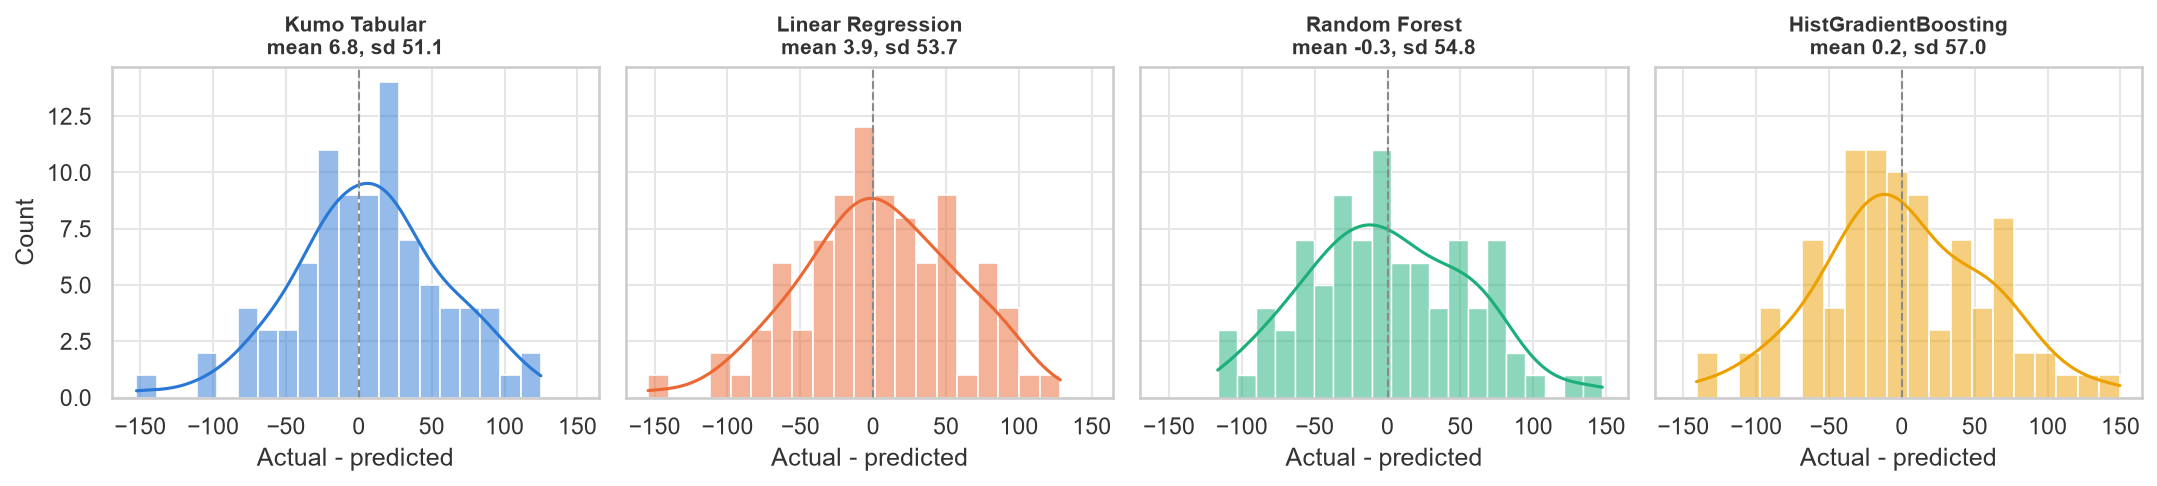
\includegraphics[width=0.92\textwidth]{regression_residuals.png}
\caption{Residual distributions (actual minus predicted) on the first regression split, with mean and standard deviation per model.}
\label{fig:residuals}
\end{figure*}

\emph{Predictive intervals.} Because Kumo Tabular returns 999 quantiles, it also provides predictive intervals at no extra cost. The nominal 90\% interval $[q_{0.05},q_{0.95}]$ covered $93.3\%\pm3.3\%$ of test targets on average, with a mean width of $174.2\pm7.8$ (Fig.~\ref{fig:intervals}). Coverage ranged from 87.6\% to 95.5\% across splits, so the intervals are approximately calibrated on these data, slightly conservative on average, and below nominal on one split. None of the baselines provides intervals without additional modelling.

\begin{figure}[t]
\centering
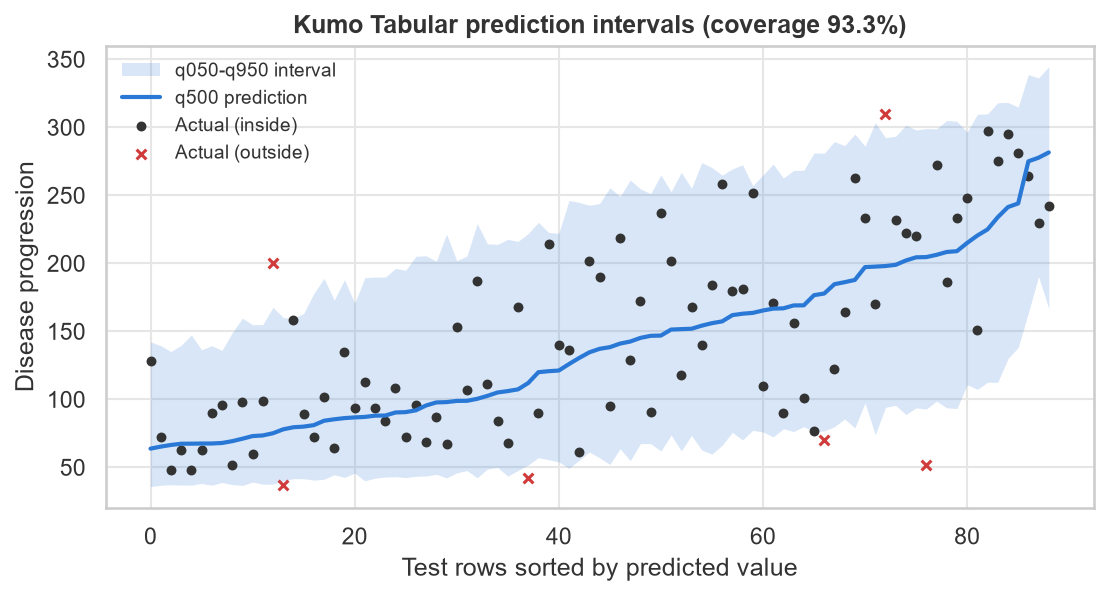
\includegraphics[width=\columnwidth]{regression_kumo_intervals.png}
\caption{Kumo Tabular median prediction and nominal 90\% interval for the test rows of the first regression split, sorted by prediction. Crosses mark targets outside the interval.}
\label{fig:intervals}
\end{figure}

\emph{Choice of point estimate.} The median minimises expected absolute error, while the mean minimises squared error \cite{gneiting2007scoring}. Table~\ref{tab:point} compares the median with the average over the 999 quantiles, which approximates the predictive mean, using the stored outputs of the same runs. The mean lowered RMSE and raised $R^2$ slightly, while the median kept the lower MAE, consistent with theory. The median is retained as the reported point prediction.

\begin{table}[t]
\centering
\caption{Kumo Tabular regression point estimates, averaged over the five splits.}
\label{tab:point}
\begin{tabular}{lccc}
\toprule
Point estimate & MAE & RMSE & $R^2$ \\
\midrule
Median $q_{0.5}$ (reported) & \textbf{42.48} & 52.88 & 0.503 \\
Mean of quantiles & 42.54 & \textbf{52.35} & \textbf{0.513} \\
\bottomrule
\end{tabular}
\end{table}

\subsection{Paired statistical analysis}
Table~\ref{tab:per_split} lists accuracy and $R^2$ per split, and Table~\ref{tab:paired} and Fig.~\ref{fig:paired} summarise the paired comparison with the strongest baseline. In classification, Kumo Tabular was better on all five splits for accuracy, recall and F1, and never worse on any split for any metric. The consistency is clear, but the evidence is weak in formal terms. The naive paired $t$-test gives $p<0.05$ for accuracy, recall and F1. After the correction for overlapping training sets, only recall remains below 0.05 ($p_{\mathrm{corr}}=0.016$, 95\% CI $[0.009,0.048]$), and after Holm adjustment across the five classification metrics no result is significant (smallest adjusted $p=0.081$). The Wilcoxon test reaches its design minimum of 0.0625 for the three metrics with five wins.

In regression, Kumo Tabular had the lower MAE on four splits but the better RMSE and $R^2$ on only three, and all corrected intervals include zero by a wide margin. The mean $R^2$ advantage of $0.007$ is small compared with the split-to-split standard deviation of the paired difference, $0.028$. On the full diabetes training set, Kumo Tabular and linear regression are therefore statistically indistinguishable in this study.

\begin{table}[t]
\centering
\caption{Per-split results of Kumo Tabular and the strongest baseline. Seeds define the train/test partition shared by all models.}
\label{tab:per_split}
\setlength{\tabcolsep}{4pt}
\begin{tabular}{ccccc}
\toprule
& \multicolumn{2}{c}{Accuracy} & \multicolumn{2}{c}{$R^2$} \\
\cmidrule(lr){2-3}\cmidrule(lr){4-5}
Seed & Kumo & Logistic Reg. & Kumo & Linear Reg. \\
\midrule
42 & 0.991 & 0.965 & 0.499 & 0.453 \\
43 & 1.000 & 0.991 & 0.556 & 0.542 \\
44 & 0.974 & 0.965 & 0.524 & 0.525 \\
45 & 0.991 & 0.982 & 0.486 & 0.519 \\
46 & 0.991 & 0.982 & 0.451 & 0.441 \\
\bottomrule
\end{tabular}
\end{table}


\begin{table*}[t]
\centering
\caption{Paired comparison of Kumo Tabular with the strongest baseline over the five splits. $\overline{d}$ is the mean advantage of Kumo (positive favours Kumo for every metric), $s_d$ its standard deviation. The corrected test and interval use the Nadeau--Bengio variance correction for overlapping training sets; Holm adjustment is applied within each task. No result is significant at $\alpha=0.05$ after adjustment.}
\label{tab:paired}
\setlength{\tabcolsep}{4.5pt}
\begin{tabular}{llcccccccc}
\toprule
Task & Metric & W/T/L & $\overline{d}$ & $s_d$ & Corrected 95\% CI & $p_{\mathrm{naive}}$ & $p_{\mathrm{corr}}$ & $p_{\mathrm{corr}}^{\mathrm{Holm}}$ & $p_{\mathrm{Wilcoxon}}$ \\
\midrule
Classification & Accuracy & 5/0/0 & 0.0123 & 0.0078 & [$-$0.0023, 0.0269] & 0.025 & 0.080 & 0.313 & 0.062 ($n$=5) \\
 & Precision & 2/3/0 & 0.0051 & 0.0111 & [$-$0.0156, 0.0258] & 0.362 & 0.531 & 0.535 & 0.500 ($n$=2) \\
 & Recall & 5/0/0 & 0.0286 & 0.0106 & [0.0087, 0.0484] & 0.004 & 0.016 & 0.081 & 0.062 ($n$=5) \\
 & F1 & 5/0/0 & 0.0172 & 0.0109 & [$-$0.0031, 0.0376] & 0.024 & 0.078 & 0.313 & 0.062 ($n$=5) \\
 & ROC-AUC & 4/1/0 & 0.0030 & 0.0034 & [$-$0.0034, 0.0094] & 0.126 & 0.267 & 0.535 & 0.125 ($n$=4) \\
\midrule
Regression & MAE & 4/0/1 & 1.27 & 1.10 & [$-$0.78, 3.32] & 0.061 & 0.161 & 0.484 & 0.125 ($n$=5) \\
 & RMSE & 3/0/2 & 0.39 & 1.43 & [$-$2.28, 3.07] & 0.573 & 0.704 & 1.000 & 0.625 ($n$=5) \\
 & $R^2$ & 3/0/2 & 0.007 & 0.028 & [$-$0.046, 0.060] & 0.603 & 0.727 & 1.000 & 0.625 ($n$=5) \\
\bottomrule
\end{tabular}
\end{table*}


\begin{figure*}[t]
\centering
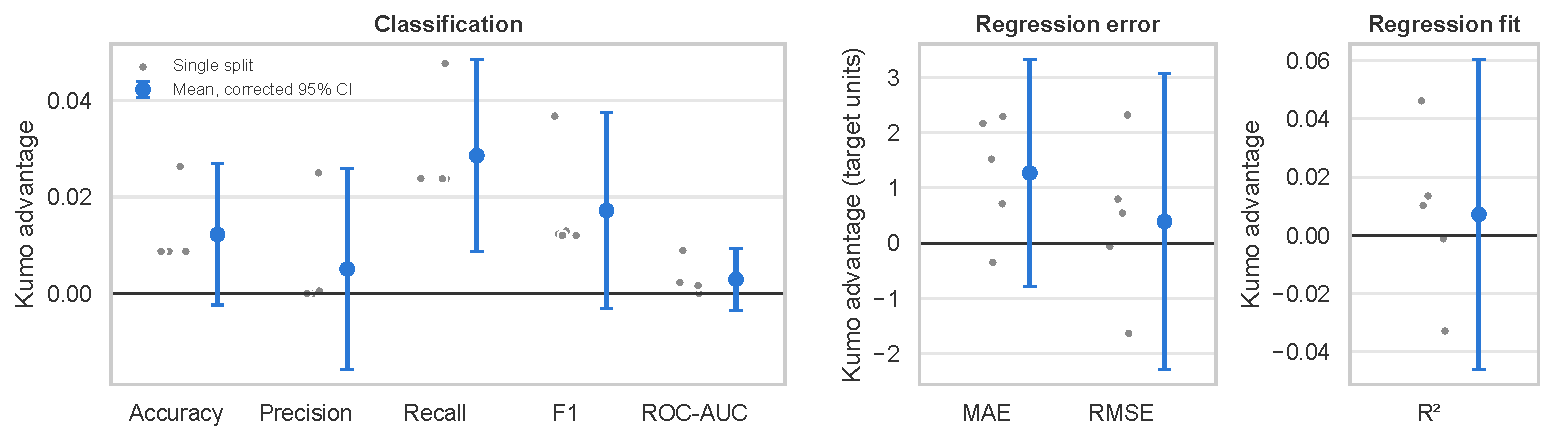
\includegraphics[width=0.94\textwidth]{paired_differences.pdf}
\caption{Paired advantage of Kumo Tabular over the strongest baseline (logistic regression for classification, linear regression for regression) on each of the five splits (grey) with the mean and the Nadeau--Bengio corrected 95\% confidence interval (blue). Positive values favour Kumo Tabular for every metric, including MAE and RMSE.}
\label{fig:paired}
\end{figure*}

\subsection{Training-size study}
Tables~\ref{tab:study_classification} and~\ref{tab:study_regression} and Fig.~\ref{fig:study} show how performance changes with the number of labelled rows. The two tasks behave differently.

In regression, Kumo Tabular was far more stable than linear regression when data was scarce. With 25 training rows it reached $R^2=0.429\pm0.058$, compared with $0.075\pm0.304$ for linear regression, which must estimate eleven coefficients from 25 noisy targets, and $0.388\pm0.127$ for random forests. Kumo Tabular remained the best regressor up to 100 rows; at 200 rows it was level with linear regression.

In classification there was no such small-data advantage. Logistic regression slightly exceeded Kumo Tabular at 25 rows ($0.956$ versus $0.950$ accuracy) and the two were level at 50 and 100 rows; Kumo Tabular pulled ahead only from 200 rows onwards. Histogram gradient boosting produced constant predictions at 25 rows (accuracy $0.632$, ROC-AUC $0.500$), because its default minimum of 20 samples per leaf leaves no room for a split. This reflects the default configuration rather than the capability of boosting.

\begin{table}[t]
\centering
\caption{Classification accuracy by training-set size (mean $\pm$ standard deviation over three seeds; full test split).}
\label{tab:study_classification}
\setlength{\tabcolsep}{3pt}
\begin{tabular}{rcccc}
\toprule
$n$ & Kumo Tabular & Logistic Reg. & Random Forest & HistGB \\
\midrule
25 & 0.950\,{\scriptsize$\pm$0.027} & \textbf{0.956}\,{\scriptsize$\pm$0.023} & 0.930\,{\scriptsize$\pm$0.018} & 0.632\,{\scriptsize$\pm$0.000} \\
50 & \textbf{0.953}\,{\scriptsize$\pm$0.051} & \textbf{0.953}\,{\scriptsize$\pm$0.022} & 0.933\,{\scriptsize$\pm$0.044} & 0.909\,{\scriptsize$\pm$0.035} \\
100 & \textbf{0.956}\,{\scriptsize$\pm$0.040} & \textbf{0.956}\,{\scriptsize$\pm$0.026} & 0.939\,{\scriptsize$\pm$0.015} & 0.944\,{\scriptsize$\pm$0.051} \\
200 & \textbf{0.985}\,{\scriptsize$\pm$0.013} & 0.971\,{\scriptsize$\pm$0.013} & 0.947\,{\scriptsize$\pm$0.009} & 0.947\,{\scriptsize$\pm$0.009} \\
400 & \textbf{0.982}\,{\scriptsize$\pm$0.015} & 0.974\,{\scriptsize$\pm$0.015} & 0.953\,{\scriptsize$\pm$0.018} & 0.956\,{\scriptsize$\pm$0.009} \\
455 & \textbf{0.988}\,{\scriptsize$\pm$0.013} & 0.974\,{\scriptsize$\pm$0.015} & 0.959\,{\scriptsize$\pm$0.013} & 0.959\,{\scriptsize$\pm$0.010} \\
\bottomrule
\end{tabular}
\end{table}


\begin{table}[t]
\centering
\caption{Regression $R^2$ by training-set size (mean $\pm$ standard deviation over three seeds; full test split).}
\label{tab:study_regression}
\setlength{\tabcolsep}{3pt}
\begin{tabular}{rcccc}
\toprule
$n$ & Kumo Tabular & Linear Reg. & Random Forest & HistGB \\
\midrule
25 & \textbf{0.429}\,{\scriptsize$\pm$0.058} & 0.075\,{\scriptsize$\pm$0.304} & 0.388\,{\scriptsize$\pm$0.127} & $-$0.097\,{\scriptsize$\pm$0.087} \\
50 & \textbf{0.437}\,{\scriptsize$\pm$0.019} & 0.331\,{\scriptsize$\pm$0.137} & 0.418\,{\scriptsize$\pm$0.008} & 0.348\,{\scriptsize$\pm$0.063} \\
100 & \textbf{0.486}\,{\scriptsize$\pm$0.045} & 0.467\,{\scriptsize$\pm$0.076} & 0.433\,{\scriptsize$\pm$0.024} & 0.410\,{\scriptsize$\pm$0.043} \\
200 & 0.505\,{\scriptsize$\pm$0.085} & \textbf{0.506}\,{\scriptsize$\pm$0.060} & 0.438\,{\scriptsize$\pm$0.057} & 0.391\,{\scriptsize$\pm$0.069} \\
353 & \textbf{0.526}\,{\scriptsize$\pm$0.028} & 0.507\,{\scriptsize$\pm$0.048} & 0.440\,{\scriptsize$\pm$0.024} & 0.406\,{\scriptsize$\pm$0.030} \\
\bottomrule
\end{tabular}
\end{table}


\begin{figure*}[t]
\centering
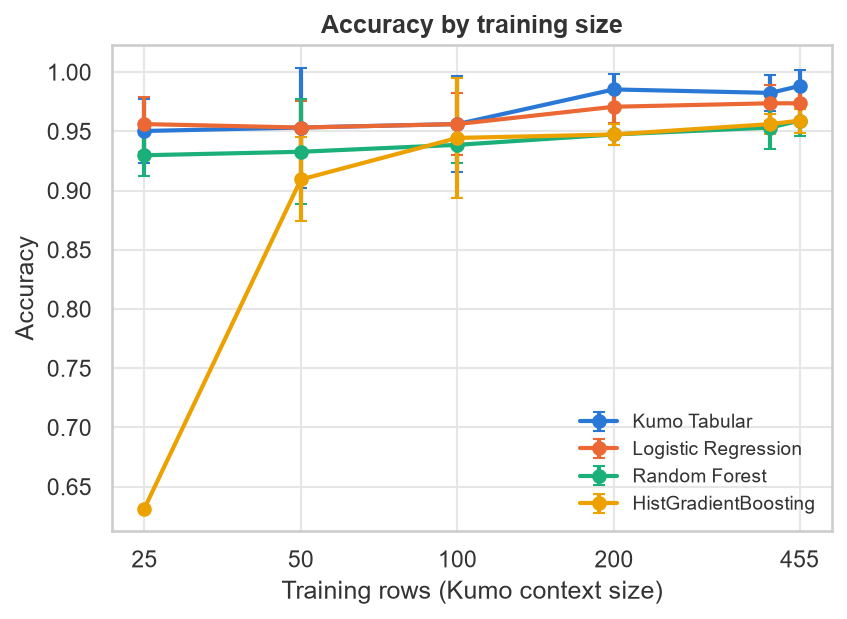
\includegraphics[width=0.45\textwidth]{classification_sample_size_accuracy.png}\hspace{0.03\textwidth}
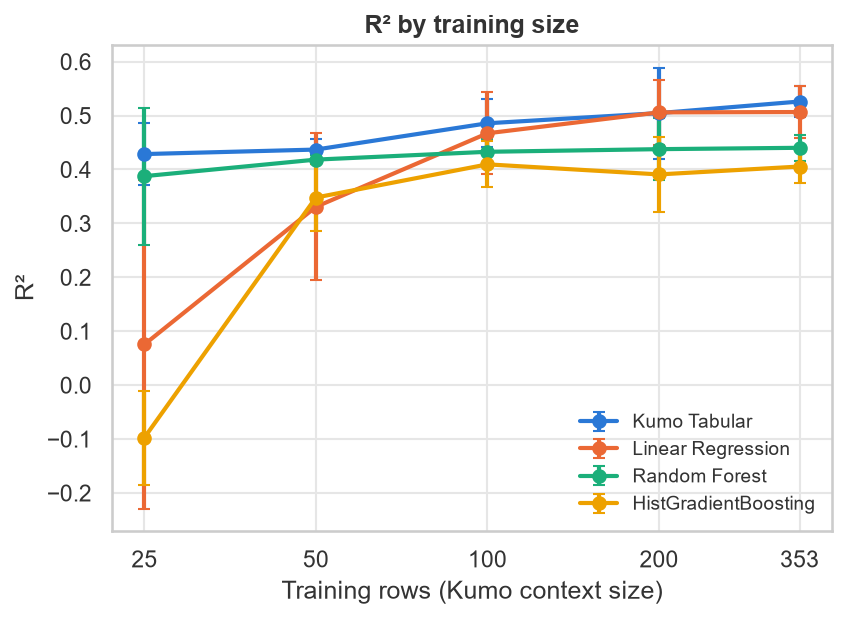
\includegraphics[width=0.45\textwidth]{regression_sample_size_r2.png}
\caption{Classification accuracy (left) and regression $R^2$ (right) as a function of the number of training rows, which is also the Kumo Tabular context size. Points show the mean over three seeds, error bars one standard deviation. The horizontal axis is logarithmic; in the left panel the 400-row point is plotted without its own tick label.}
\label{fig:study}
\end{figure*}

\subsection{Runtime}
Fig.~\ref{fig:runtime} and the last columns of Tables~\ref{tab:classification} and~\ref{tab:regression} compare runtimes. Per split, Kumo Tabular needed $1.10$\,s for classification and $0.63$\,s for regression on the GTX 980M, compared with $0.019$\,s and $0.003$\,s for logistic and linear regression, roughly 60 and 220 times more. These ratios are sensitive to the very short baseline timings: in a complete re-run of both experiments on the same machine, all metrics were identical, but the per-split times were $1.22$\,s versus $0.052$\,s for classification and $0.68$\,s versus $0.023$\,s for regression, ratios of about 23 and 30. The published Kaggle notebooks, run on a Tesla T4 GPU with float16 autocast, measured 0.41 to 0.52\,s per split for Kumo Tabular and ratios of about 6 to 49 relative to the linear models. The cost ratio therefore depends strongly on hardware and on noise in millisecond-scale timings; across all measured runs it ranged from about 6 to 220. On the GTX 980M, Kumo Tabular was comparable to a 500-tree random forest on the CPU and slower than histogram gradient boosting. In the training-size study, Kumo Tabular prediction time grew from $0.46$\,s with 25 context rows to $1.11$\,s with 455 rows for classification, and from $0.44$\,s to $0.64$\,s for regression, so a fixed overhead dominates at these sizes. The GPU used here is old and could not use reduced-precision arithmetic; absolute times on current hardware are expected to be lower, but the cost of a forward pass that processes the whole context will remain large relative to applying a fitted linear model.

\begin{figure*}[t]
\centering
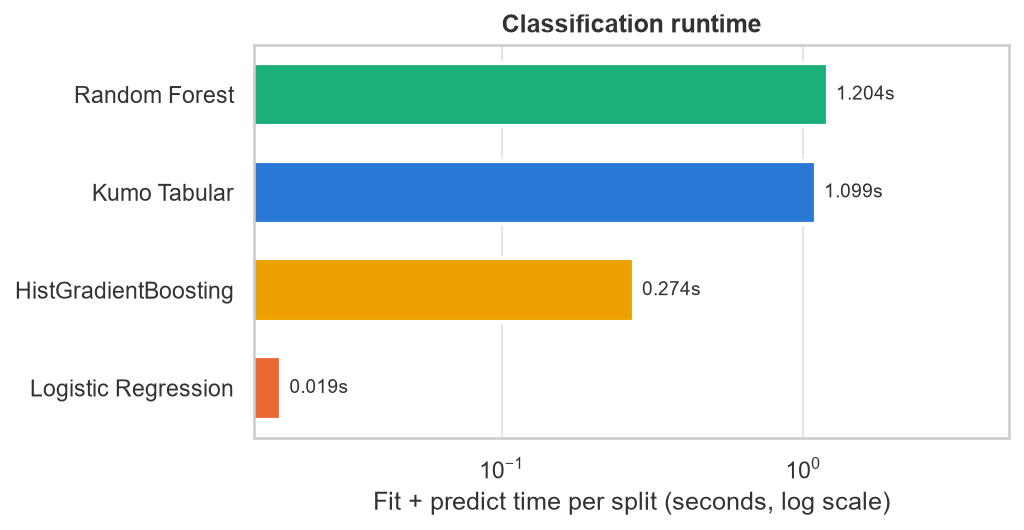
\includegraphics[width=0.45\textwidth]{classification_inference_time.png}\hspace{0.03\textwidth}
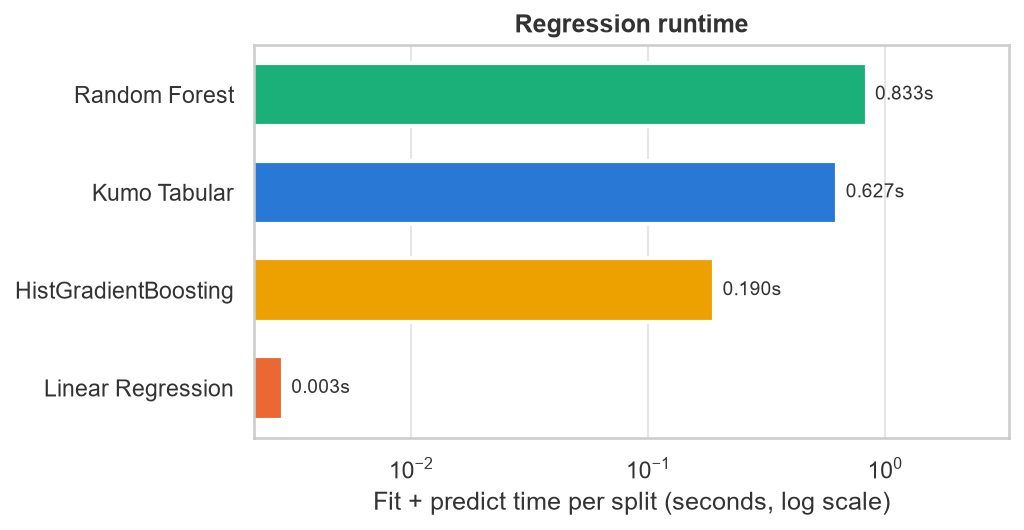
\includegraphics[width=0.45\textwidth]{regression_inference_time.png}
\caption{Mean fit plus prediction time per split for classification (left) and regression (right), logarithmic scale. Kumo Tabular ran on the GPU, the baselines on the CPU.}
\label{fig:runtime}
\end{figure*}

\subsection{Error analysis}
Across the five classification test sets, 38 split-specific test cases were misclassified by at least one model, and 4 of them by all four models. Kumo Tabular made 6 errors: 4 of these were among the cases that every model misclassified, three of them malignant tumours to which Kumo Tabular assigned a malignancy probability below 0.07; one error was shared only with the random forest; and one was made by Kumo Tabular alone. Most of its remaining errors therefore concern cases that appear genuinely ambiguous in the feature space rather than failures specific to the pretrained model.

\section{Discussion}

\emph{Where Kumo Tabular helps.} Without any tuning or feature engineering, the smallest Kumo Tabular checkpoint matched or exceeded every classical baseline on both tasks. In classification its advantage was consistent across splits and concentrated in recall of the positive class, which is the operationally important error on this dataset. In regression its most useful property was robustness with very few labelled rows, where it avoided the high variance of an unregularised linear model, and its quantile output provided reasonably calibrated intervals for free. These observations agree in direction with reports that pretrained in-context learners are strong on small tables \cite{hollmann2023tabpfn,hollmann2025tabpfn}.

\emph{Where it does not.} The size of the advantage was modest. On both full tasks the strongest baseline was a linear model, and the remaining differences are of the order of one test row in classification and within noise in regression. On small classification training sets logistic regression was as accurate as Kumo Tabular. Both datasets are low-dimensional, fully numerical, free of missing values and well suited to linear models; they leave little room for a more expressive model and test none of the capabilities, such as handling categorical features or missing values, that the model was designed for.

\emph{Cost of in-context learning.} The distinction between \eqref{eq:erm} and \eqref{eq:icl} has practical consequences. A classical model concentrates its cost in fitting and then predicts almost instantly; Kumo Tabular has no fitting cost but processes the full context on every prediction call. For a one-off analysis of a small table this trade-off is favourable, since no model selection is needed. For repeated scoring or latency-sensitive use, the per-call cost and the GPU dependency matter, unless context caching, which the architecture supports according to its developers, is used.

\emph{Practical implication.} For small numerical tables, Kumo Tabular is a reasonable default that is unlikely to perform worse than untuned classical models and can be better when labelled data is scarce. It should not be assumed to outperform a well-chosen linear model by a meaningful margin, and claims of superiority on a specific dataset require more splits or repetitions than were used here.

\section{Threats to Validity}

\emph{Statistical conclusion validity.} Five splits of 114 and 89 test rows provide limited power; one classification error changes accuracy by about 0.009. Resampled splits are dependent, and the corrected test of \eqref{eq:corrected} is itself an approximation \cite{nadeau2003inference}. Several metrics were tested per task; the Holm adjustment addresses this within tasks but not across the training-size study, which is reported descriptively only.

\emph{Internal validity.} All models used identical splits and the implementation guards against target leakage, which is covered by unit tests. Baselines were not tuned, while Kumo Tabular brings tuning-free defaults by design; tuned boosting or regularised linear models could narrow or reverse some differences. Runtimes compare a GPU pipeline with CPU pipelines and are specific to the hardware used.

\emph{External validity.} Only two small, clean, widely studied datasets were used, with no categorical features and no missing values, and only the smallest of three checkpoints was evaluated. Kumo Tabular was reportedly pretrained on synthetic data only \cite{nvidia_kumo_blog}, which makes memorisation of these datasets unlikely, but the results cannot be generalised to larger, high-dimensional or heterogeneous tables, to the larger checkpoints, or to other domains.

\emph{Construct validity.} Threshold-based metrics use a fixed 0.5 threshold; in a diagnostic setting the threshold would be chosen for a target sensitivity. The datasets serve as benchmarks; no conclusion about clinical use is drawn or supported.

\section{Limitations and Future Work}

The main limitations are the small number of datasets and splits, the absence of hyperparameter tuning for the baselines, the evaluation of a single checkpoint size, and runtimes measured on one older laptop GPU. Future work should (i) use repeated cross-validation on a larger and more diverse collection of tables, including categorical features and missing values; (ii) compare against tuned gradient boosting and against other tabular foundation models such as TabPFN \cite{hollmann2025tabpfn} and TabICL \cite{qu2025tabicl}; (iii) evaluate the medium and large checkpoints and reduced-precision inference on current GPUs; (iv) study probability calibration and threshold selection in classification; and (v) measure the benefit of context caching for repeated predictions.

\section{Conclusion}

This study compared NVIDIA Kumo Tabular with logistic or linear regression, random forests and histogram gradient boosting on two small public datasets under a controlled and reproducible protocol. Used without tuning, the smallest Kumo Tabular checkpoint achieved the best mean on every metric, never lost to the strongest baseline on any classification split, and was markedly more robust than linear regression with very few training rows. At the same time, its advantage over linear models on the full tasks was small and not statistically significant once the dependence between splits and multiple comparisons were accounted for, it offered no advantage over logistic regression on small classification training sets, and its prediction time per split was about 6 to 220 times that of the linear models, depending on hardware and run. Pretrained in-context learning is therefore a credible and convenient option for small tables, but on these benchmarks it is an incremental rather than a decisive improvement over well-chosen classical models.

\section*{Data and Code Availability}
The implementation, configuration, raw per-split results, figures and the scripts that generate every table and statistic in this paper are available at \url{https://github.com/noyonahmedjoy/Kumo-Tabular} \cite{project_repo}. Self-contained notebooks reproducing the experiments are published on Kaggle \cite{project_kaggle}. Run by the author on Kaggle (Tesla T4 GPU, PyTorch 2.11, float16 autocast), their stored outputs reproduce all reported results for Kumo Tabular, logistic and linear regression and random forests at the precision reported here; results for histogram gradient boosting differ slightly (for example, classification accuracy 0.960 instead of 0.967), presumably because of a different scikit-learn version. Kumo Tabular weights are provided by NVIDIA under the OpenMDW 1.1 licence \cite{nvidia_kumo_card}.

\section*{Acknowledgment}
In accordance with IEEE policy on AI-generated content, the author discloses the use of two AI systems. Claude Opus 5.5 (Anthropic), accessed through the Claude Code desktop application, was used extensively. Working from written specifications provided by the author, it wrote the software in the accompanying repository (data loading, model wrappers, benchmarking, evaluation, plotting, unit tests and notebook generation), executed the local experiments, and produced all figures and tables from the saved experiment outputs, including the diagram in Fig.~\ref{fig:paradigms}. It performed the statistical analysis described in Section~\ref{sec:stats}, searched for and verified the references against bibliographic databases, and drafted the complete text of this article, including the abstract and every section; AI-generated text is therefore not confined to particular sections. ChatGPT (OpenAI; model version not recorded) was used for research planning, for preparing the written specifications given to Claude, for review assistance, and for drafting the author biography. ChatGPT did not generate the experimental results, figures, tables or statistical analyses. The author defined the research topic, objectives, datasets, models and evaluation requirements, ran the published Kaggle notebooks, reviewed the project and the manuscript, and takes full responsibility for the content of this article.

\begingroup
\raggedright
\bibliographystyle{IEEEtran}
\bibliography{references}
\endgroup

\begin{IEEEbiographynophoto}{MD. Noyon Ahmed Joy}
is an independent researcher based in Bangladesh. His research interests include machine learning, tabular data modeling, and empirical evaluation of predictive methods. His work focuses on reproducible experimentation and benchmarking machine learning approaches on structured datasets.
\end{IEEEbiographynophoto}

\EOD

\end{document}
